\documentclass{mwart} 
\usepackage[polish]{babel} 
\usepackage[utf8]{inputenc} 
\usepackage{polski} 
\usepackage[T1]{fontenc} 
\usepackage{graphicx}

\usepackage[margin=1cm]{geometry}




\frenchspacing 

\usepackage{indentfirst} 
\title{\Huge{Sprawozdanie z laboratorium nr 5 \\
Algorytmy Sortujące -QUICKSORT }}
\author{Agnieszka Wiśniewska, nr albumu: 200466}
\date{30.03.2014} 
\begin{document}

\maketitle

\section{Opis działania algorytmu}
Algorytm sortowania szybkiego opiera się na strategii "dziel i zwyciężaj". Proces quicksort-u można podzielić na następujące etapy:
\begin{itemize}
\item{\textbf{Dziel}
- na początku dzieli sortowaną tablicę na dwie tak, aby wszystkie elementy leżące w pierwszej tablicy były mniejsze od wszystkich elementów drugiej tablicy.}
\item{\textbf{Zwyciężaj}
- każdą z tablic jest sortowana rekurencyjnie tym samym algorytmem.}
\item{\textbf{Połącz}
- ostatnim krokiem jest połączenie tablic w jedną posortowaną.}
\section{Złożoność obliczeniowa algorytmu}
Złożoność obliczeniowa została zbadana dla dwóch przypadków - gdy tablica jest wstępnie posortowana oraz gdy elementy tablicy są losowe.
Wyniki zostały przedstawione na wykresie \ref{trend}.
\end{itemize}

\begin{figure}[!htp]
\centering
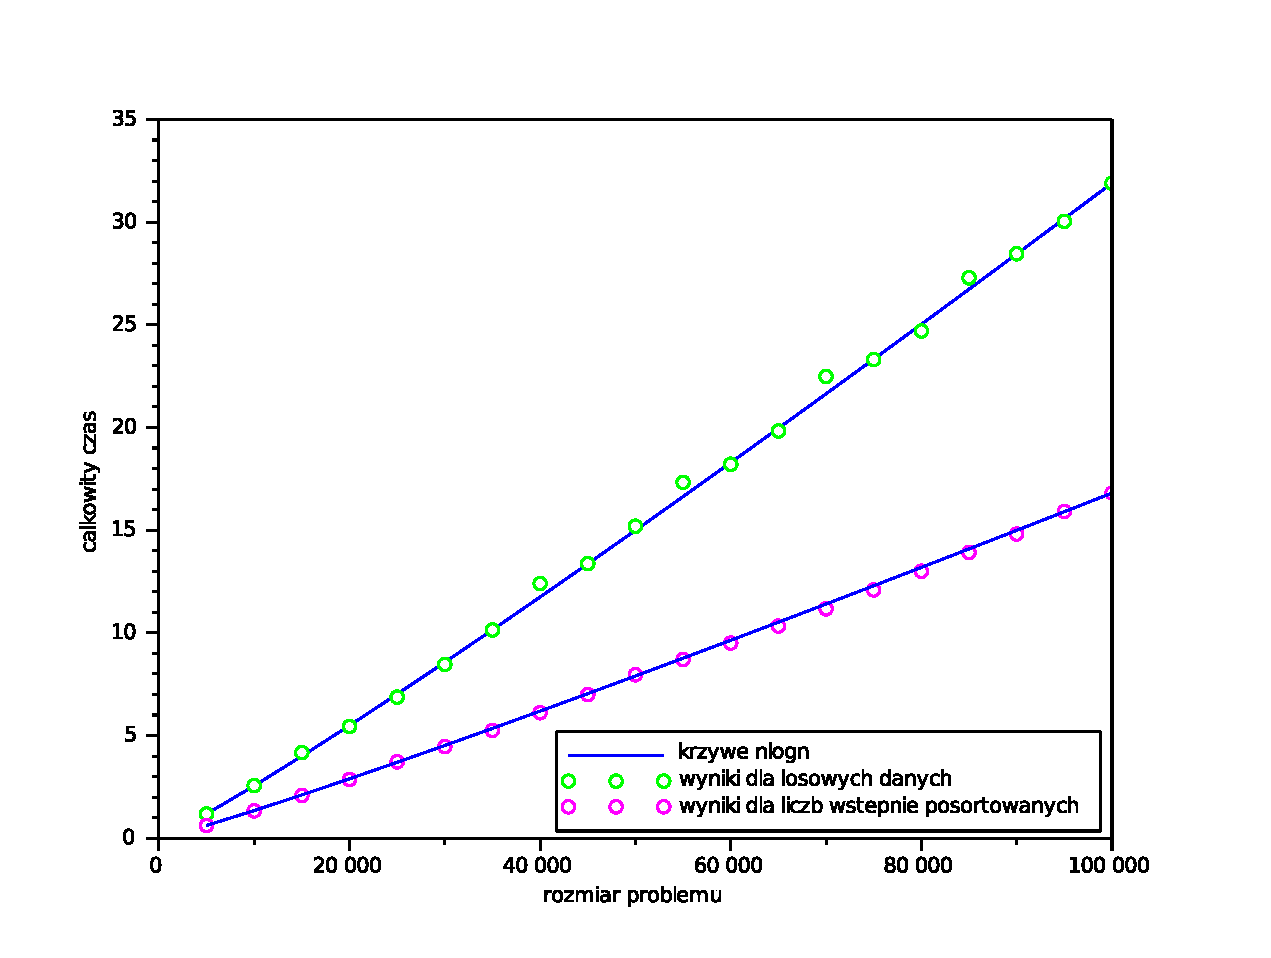
\includegraphics[width=0.8\textwidth]{files/trend.pdf}
\caption{Zależność czasu wykonywania algorytmu od rozmiaru problemu dla sortowania szybkiego.\label{trend}} 
\end{figure}
\newpage
\section{Podsumowanie i wnioski}
Jak widać na powyższym wykresie zależności czasu od rozmiaru problemu pokrywają się z krzywymi dopasowania nlogn\footnote{są to funkcje przemnożona przez odpowiednio dobraną stałą}. Wynika z tego, że obu sprawdzanych przypadkach złożoność obliczeniowa wynosi O(nlogn). W szczegolnych przypadkach (np.: w przypadku niekorzystnego ułożenia danych) złożoność obliczeniowa algorytmu może wynosić O($n^{2}$) jest to jednak przypadek, który przy takiej implementacji algorytmu nie powinien wystąpić.





\end{document}